\subsection{並び替え機能}
並び替え機能は，以下のような機能から構成されている．

\begin{itemize}
    \item 距離順
    \item リアクション数順
    \item 新着順
\end{itemize}

\subsubsection{距離順}

距離順機能では，現在地または任意の場所からの距離が近い順にピンを並べ替えて表示する．

操作の流れとしては，まず並び替え機能をクリックし，並び替え項目を展開して表示する．
その後，「距離順」を選択すると，データベースにアクセスし，投稿内容を取得して距離順に並び替え，画面に表示する．

\begin{figure}[H]
        \centering
        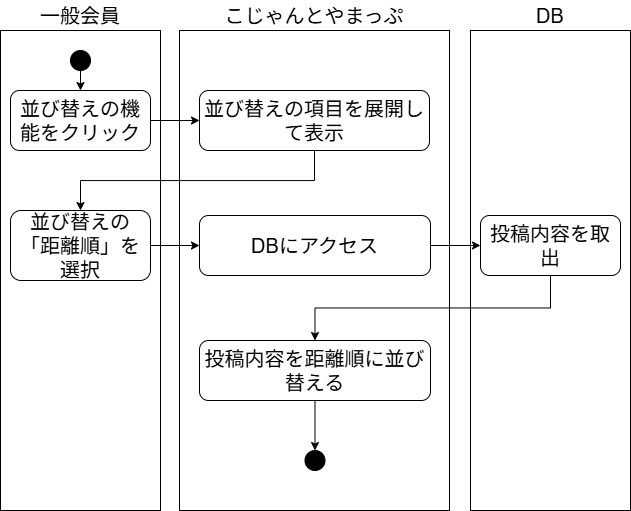
\includegraphics[scale=0.5]{sections/fig_sort_general/sort_gen1.jpg}
        \caption{距離順}

        %\label{}

\end{figure}